\chapter{Platforma Zynq-7000}
\label{platforma}

Układ \emph{ZYBO} jest przedstawicielem rodziny układów \emph{SoC} (\emph{ang}. System-on-a-chip) \emph{Zynq-7000}. \emph{SoC} to układy scalone integrujące wszystkie elementy budowy układów elektronicznych, powszechnie wykorzystywane do projektowania systemów wbudowanych. Centralną część układu rodziny \emph{Zynq-7000} stanowi dwurdzeniowy procesor o architekturze ARM w wersji Cortex-A9. \cite{zynq-homepage} Układ \emph{ZYBO} wyposażony jest ponadto w 512 MB pamięci RAM, złącza HDMI i VGA do transmisji obrazu, gniazda Jack do przesyłu dźwięku, gniazdo USB oraz slot pamięci MicroSD. Komunikacja sieciowa jest możliwa dzięki implementacji stosu TCP/IP i obecności gniazda RJ-45. \cite{zynq-datasheet}

Układy rodziny \emph{Zynq-7000} są stosowane w aplikacjach systemów wsparcia kierowców (\emph{ADAS}), systemach wizyjnych wysokich rozdzielczości, cyfrowego przetwarzania sygnałów czy kryptograficznych. \cite{GuanwenZhong,MaleenAbeydeera,PawelDabal2014}

Układy rodziny \emph{Zynq-7000} są układami heterogenicznymi, łączącymi w sobie elementy klasycznego układu FPGA (PL, ang. \emph{Programmable Logic}) oraz procesora ARM (PS, ang. \emph{Processing System}). Na rysunku \ref{fig:zynq-overview} przedstawiono schemat omawianej architektury.

\begin{figure}[h]
	\centering
	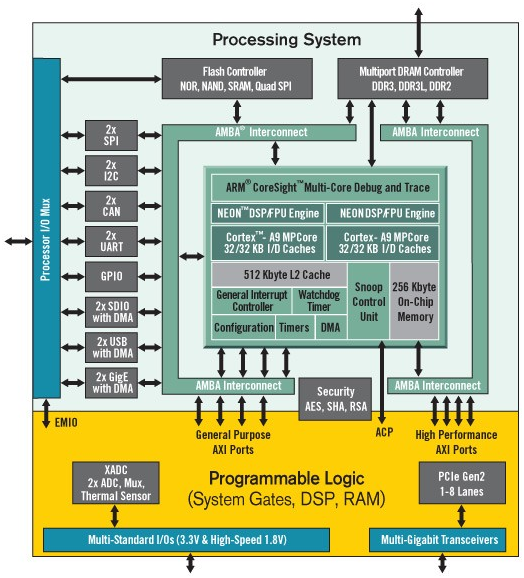
\includegraphics[width=8cm]{img/zyng-platform.png}
	\caption{Schemat architektury \emph{Zynq-7000}. (Źródło: \cite{zybo-reference-manual})}
	\label{fig:zynq-overview}
\end{figure}

Schemat przedstawia podział układu na części \emph{PL} - oznaczonej kolorem żółtym, oraz \emph{PS} - na zielono.
Architektura części programowalnej zbliżona jest do powszechnie stosowanych układów FPGA. Wyposażono ją jednak w zbiór portów umożliwiających wydajną komunikację z procesorem. Ponadto, konfiguracja tej części wykonywana jest na starcie przez procesor lub przy użyciu interfejsu JTAG i układ nie zawiera elementów pozwalających na wykorzystanie logiki programowalnej niezależnie.
Część procesorowa wyposażona jest w szereg interfejsów, w tym kontroler pamięci DDR3, interfejs komunikacji AMBA oraz zbiór interfejsów peryferyjnych.

Procesor wyposażony jest w koprocesor arytmetyczny, wspierający w obliczeniach na liczbach zmiennoprzecinkowych oraz wspiera obsługę architektury SIMD (ang. \emph{Single Instruction, Multiple Data}) - pozwalającej na przetwarzanie wielu strumieni danych przy użyciu jednego strumienia instrukcji. Zagadnienia te szerzej opisane zostały w sekcji \ref{sec:arm-neon}.

Układ wyposażony jest w kontroler pamięci DDR, obsługujący żądania dostępu ze strony zarówno procesora, jak i układu FPGA. Pamięć jest współdzielona między oboma modułami. Pozwala to na wymianę danych, do czego wykorzystywany jest standard AXI. Interfejs pozwala na transmisję pojedynczych słów danych, umożliwiając konfigurację parametrów pracy modułów algorytmicznych, jak i na transmisję o wysokiej przepustowości. Pozwala to, dzięki zastosowaniu modułu VDMA, na przesył obrazu o rozdzielczości HD z częstotliwością osiągającą wartości 680 klatek na sekundę. \cite{axi-vdma-guide} Interfejs AXI opisano szerzej w sekcji \ref{sec:axi-std}.

\section{Konfiguracja procesora}
\label{sec:arm-programming}
Centralny element architektury stanowi dwurdzeniowy procesor ARM. Jest on odpowiedzialny za przeprowadzenie konfiguracji układów logiki reprogramowalnej. Ponadto, pozwala na wykonanie dowolnego programu użytkownika. Powszechnie stosowana jest konfiguracja bare metal,w której procesor wykonuje program zaprojektowany w pełni przez użytkownika. Pozwala to na uzyskanie możliwie największej kontroli nad pracą układu, ogranicza jednak możliwości wykorzystania pełni zasobów procesora oraz utrudnia projektowanie rozbudowanych aplikacji.

W niniejszej pracy badano możliwość wykorzystania systemu operacyjnego Linux na przykładzie aplikacji systemów wizyjnych. Dzięki zastosowaniu Linuxa, możliwe staje się budowanie programów składających się z wielu modułów działających niezależnie. System ten wspiera obsługę sieci, co pozwala na wykorzystanie narzędzi komunikacji sieciowej, jak SSH \cite{ssh-protocol}, do konfiguracji i nadzorowania działania aplikacji, co opisano w sekcji \ref{sec:ssh}. Ponadto, możliwe jest wykorzystanie powszechnie dostępnych bibliotek, ułatwiających rozwój aplikacji w krótkim czasie. Zagadnienie to badano na przykładzie biblioteki OpenCV \cite{opencv-library}, udostępniającej narzędzia przetwarzania obrazów, co opisano w sekcji \ref{sec:opencv-lib}.

Zbadano możliwość wykorzystania systemu PetaLinux, rozwijanego przez organizację Xilinx, jak i podstawowej wersji systemu oraz dystrybucji bazującej na Ubuntu Core.

\section{Petalinux}
Firma Xilinx zapewnia dostęp do zbioru narzędzi \emph{PetaLinux Tools} \cite{petalinux-tools}, umożliwiających przeprowadzenie procesu konfiguracji, budowania i uruchamiania systemu Linux na platformie Zynq. Dzięki zintegrowaniu koniecznych narzędzi w jednym pakiecie, proces ten jest w dużej części zautomatyzowany i ogranicza interakcję z programistą, zapewniając przy tym możliwość dowolnej konfiguracji systemu.

Celem wykorzystania omawianego pakietu narzędzi jest zbudowanie systemu operacyjnego gotowego do uruchomienia i umożliwiającego szybką rekonfirugację zarówno elementów logiki reprogramowalnej jak i samego systemu operacyjnego.

Pakiet wymaga dostarczenia zewnętrznych zależności, w tym narzędzi umożliwiających budowanie systemu - kompilatora, generatora parserów, systemu budowania - oraz zbioru narzędzi programistycznych i konfiguracyjnych.
W przypadku dystrybucji Debian, zależności mogą być zainstalowane poleceniem:

\begin{lstlisting}[breaklines=true]
apt-get install tofrodos iproute2 gawk gcc git make net-tools libncurses5-dev tftpd zlib1g-dev libssl-dev flex bison libselinux1
\end{lstlisting}

W przypadku pracy na systemie wspierającym architekturę 64-bitową, konieczne jest również zainstalowanie bibliotek programistycznych dla architektury 32-bitowej.

\begin{lstlisting}[breaklines=true]
dpkg --add-architecture i386
apt-get update
apt-get install libc6:i386 libncurses5:i386 libstdc++6:i386
apt-get install libgtk2.0-0:i386 libxtst6:i386 gtk2-engines-murrine:i386 lib32stdc++6 libxt6:i386 libdbus-glib-1-2:i386 libasound2:i386
\end{lstlisting}

Praca z pakietem wymaga ponadto wykorzystania oprogramowania \emph{Vivado Design Suite} \cite{vivado-home} do zaprojektowania układu połączeń logiki reprogramowalnej oraz \emph{Xilinx SDK} \cite{xsdk-home} do kompilacji programów uruchamianych w środowisku systemu operacyjnego układu.

Pierwszym krokiem jest wykonanie projektu w pakiecie \emph{Vivado}. Szczegóły procesu opisano w dodatku \ref{sec:vivado-conf}. Wyeksportowany projekt jest konieczny do przeprowadzenia procesu budowania systemu.

Proces konfiguracji projektu PetaLinux opisano w dodatku \ref{sec:petalinux-config}.

Pakiet udostępnia możliwość dodania do budowanego systemu zbioru programów i bibliotek. Dostępne jest kilkaset pakietów oprogramowania dostępnego na zasadach wolnych licencji, w tym biblioteki do przetwarzania obrazów. Ponadto, pakiet umożliwia dodanie własnoręcznie zbudowanych aplikacji. Pozwala to na integrację etapu projektowania aplikacji oraz budowy i uruchamiania systemu operacyjnego w jednym procesie.

Projekt PetaLinux jest niezależny od projektu Vivado i może powstawać równolegle. Zmiany w strukturze modułów logiki reprogramowalnej wymagają ponownego zbudowania plików wynikowych systemu, jednak proces ten został wydzielony z oprogramowania Vivado. Pozwala to na wykorzystanie jednego projektu opisującego logikę współpracującego z aplikacjami bare metal i systemowymi. 

Proces budowania systemu jest czasochłonny, na etapie prototypowania aplikacji praktyczne jest zastosowanie oprogramowania pracującego w trybie bare metal. Pozwala to na przeprowadzanie procesu debugowania aplikacji bezpośrednio z poziomu oprogramowania Vivado/SDK. Po upewnieniu się, że sprzętowa część algorytmu działa poprawnie, zaprojektować można aplikację systemową, odpowiedzialną za komunikację, monitorowanie wykorzystanie wyników działania algorytmu w kompletnym projekcie.

\section{Inne dystrybucje systemu}
Po zapoznaniu się z możliwościami pakietu \emph{Petalinux}, zbadano również inne możliwości konfiguracji systemu operacyjnego do zastosowania na układzie \emph{ZYBO}. Wśród dostępnych opcji, zdecydowano się na zapoznanie z dystrybucją \emph{Ubuntu Core} oraz badano możliwość budowy systemu Linux ze źródeł.

\subsection{Budowa ze źródeł}
% http://jeremyherbert.net/get/digilent_zybo_zynq_getting_started
Wykorzystanie pakietu PetaLinux związane jest z ograniczeniem dostępności projektu do środowisk, w których pakiet narzędzi jest dostępny. W przypadku konieczności uruchomienia projektu na systemie nie wspieranym przez twórców oprogramowania lub potrzeby wprowadzenia dużych zmian w kodzie źródłowym systemu i konfiguracji, konieczne może być przeprowadzenie pełnego procesu budowania samodzielnie. Takie podejście pozwala również na pełne zrozumienie kolejnych kroków procesu konfiguracji.

Proces budowy systemu składa się z kilku kroków. Wymagane jest zaprojektowanie połączeń logiki reprogramowalnej i wykorzystanie wynikowego pliku binarnego na etapie budowy.

Konieczne jest zbudowanie dwóch programów rozruchowych. Pierwszy z nich - FSBL (ang. \emph{First Stage Boot Loader}) - odpowiada za przeprowadzenie procesu wstępnej konfiguracji procesora, kontrolera pamięci i uruchomienie drugiego programu rozruchowego. W tej roli wykorzystywany jest program U-Boot. Jego zadaniem jest przygotowanie środowiska do uruchomienia właściwego systemu operacyjnego.

Kolejny krok wymaga zbudowania struktury drzewa urządzeń (ang. \emph{device tree}). Struktura ta pozwala na zdefiniowanie i konfigurację urządzeń połączonych z procesorem, dzięki czemu mogą być one obsłużone przez system operacyjny. W przypadku układu ZYBO, wykorzystanie tej struktury pozwala na konfigurację i komunikację z elementami układu FPGA.

Po przeprowadzeniu wstępnej konfiguracji elementów systemu, możliwe jest wykonanie procesu konfiguracji, budowania i przygotowania wynikowych plików binarnych.

Opisany proces jest skomplikowany i wymaga specjalistycznej wiedzy. Dostępne są obszerne opracowania dotyczące tematu, zawierające precyzyjny opis kolejnych wymaganych kroków. \cite{zybo-zynq-getting-started,zybo-stock-linux,xilinx-build-kernel}

\subsection{Ubuntu Core}
Ubuntu Core to dystrybucja systemu Linux dedykowana do zastosowań w urządzeniach koncepcji internetu rzeczy. Dystrybucja ta oparta jest na podstawowej wersji systemu Ubuntu, przystosowana do uruchomienia na urządzeniach o ograniczonej mocy obliczeniowej.

Dzięki wykorzystaniu Ubuntu Core, możliwy jest dostęp do repozytorium oprogramowania udostępnianego przez dystrybucję. PW przeciwieństwie do dystrybucji \emph{PetaLinux}, instalowane oprogramowanie może być aktualizowane w trakcie pracy systemu. Cecha ta może być istotna w przypadku aplikacji działających przez długi czas, gdy aktualizacja oprogramowania jest korzystna ze względu na znalezione błędy lub poprawę działania w kolejnej wersji.

\subsection*{}
Zarówno wykorzystanie pakietu \emph{Petalinux Tools}, jak i obu pozostałych metod pozwala na zbudowanie w pełni funkcjonalnej dystrybucji systemu Linux i uruchomienie jej na układzie ZYBO. Każda z metod wiąże się z innymi ograniczeniami i udostępnia inne możliwości. W przypadku użycia narzędzi \emph{PetaLinux}, użytkownik uzyskuje dostęp do ograniczonego zbioru dodatkowych aplikacji, niewielkiej w porównaniu do repozytoriów udostępnianych w dystrybucji Ubuntu Core. Ponadto, aktualizacja oprogramowania może wymagać ponownego zbudowania systemu lub nie być możliwa bez aktualizacji pakietu narzędzi. 

Ponadto, dystrybucja Ubuntu Core zapewnia dostęp do aktualizacji samego systemu, pozwalając na zachowanie bezpieczeństwa działania i dostęp do poprawek kodu oprogramowania. Może to być kluczowe w przypadku wykorzystania układu ZYBO do działania przez długi czas z oczekiwaną niezawodnością.

W przypadku konieczności dostosowania kodu systemu operacyjnego do własnych potrzeb, praktyczne staje się natomiast wykorzystanie technik budowy systemu bezpośrednio ze źródeł. Ogranicza to jednak możliwości instalacji dodatkowego oprogramowania i wymaga dobrej znajomości zagadnień związanych z działaniem systemu Linux.

Pakiet \emph{PetaLinux} pozwala jednak na największą integrację z oprogramowaniem Vivado, co ułatwia prototypowanie aplikacji. Dzięki udostępnieniu repozytorium oprogramowania oraz braku konieczności ingerencji użytkownika w proces budowania systemu, wykorzystanie go jest najlepszym rozwiązaniem w większości projektów. Z tego powodu, w niniejszej pracy zdecydowano się na użycie tego rozwiązania na dalszym etapie projektu.

\section{RTOS}
System operacyjny czasu rzeczywistego (ang. \emph{RTOS - real time operating system}) to system operacyjny, którego zadaniem jest obsługa aplikacji przy zachowaniu założeń o nieprzekroczeniu maksymalnego dopuszczalnego czasu odpowiedzi programu. Pozwala to na projektowanie aplikacji, w których czas odpowiedzi ma kluczowe znaczenie, w tym systemów sterowania lub krytycznych aplikacji wizyjnych.

Dzięki zastosowaniu dwurdzeniowego procesora w układzie \emph{ZYBO}, rozważyć można zaprojektowanie rozwiązania, w których jeden z rdzeni odpowiada za wykonanie programu Linuxa, a drugi - aplikacji lub systemu czasu rzeczywistego.

Rozpatrzono możliwość uruchomienia systemu operacyjnego PetaLinux i jego współpracę z aplikacjami czasu rzeczywistego na przykładzie narzędzi OpenAMP.\cite{openamp-home} OpenAMP zapewnia interfejs umożliwiający komunikację pomiędzy programami działającymi w systemie Linux oraz aplikacjami czasu rzeczywistego, wykorzystując do tego narzędzia dostępne już w systemie.

Z punktu widzenia klasycznego systemu operacyjnego, program działający na systemie czasu rzeczywistego jest zewnętrznym zasobem, który oczekuje na zlecenie wykonania konkretnego zadania i wysyła odpowiedź.

Dzięki wykorzystaniu systemu czasu rzeczywistego FreeRTOS \cite{freeRTOS-home}, aplikacje mogą mieć dostęp do zasobów systemowych, w tym pamięci i interfejsów komunikacji.

System czasu rzeczywistego może być wykorzystany do obliczeń o krytycznym znaczeniu. W przypadku wykorzystania klasycznego systemu operacyjnego, nie jest możliwe zagwarantowanie wykonania dowolnego zadania w określonym czasie. W trakcie działania aplikacji, system może zadecydować o jej czasowym zatrzymaniu i udostępnieniu zasobów innemu z oczekujących zadań. Aplikacja działająca w czasie rzeczywistym pozwala uniknąć tego zjawiska.

System PetaLinux oferuje dostęp do modułów \texttt{RPMsg}, \texttt{remoteproc}, \texttt{virtIO}, które są wymagane do zapewnienia komunikacji z systemem czasu rzeczywistego. Udostępnione zostały również aplikacje testowe, które pozwalają na sprawdzenie poprawności działania konfiguracji.

Użycie systemu czasu rzeczywistego wymaga zmian projektowych, w tym konfiguracji dwóch instancji konsoli do komunikacji szeregowej i zdefiniowania struktury drzewa urządzeń określającej obszar pamięci dla obu systemów operacyjnych. Po zbudowaniu poprawie skonfigurowanego systemu i jego uruchomieniu, przetestowanie działania aplikacji wymaga użycia poniższych poleceń.

\begin{lstlisting}[breaklines=true]
modprobe zynq_remoteproc firmware=image_echo_test
modprobe rpmsg_user_dev_driver
echo_test
\end{lstlisting}

Uruchomione zostaną moduły odpowiedzialne za obsługę systemu czasu rzeczywistego i przeprowadzony zostanie test komunikacji.

Konfiguracja i wykorzystanie systemów czasu rzeczywistego wykracza poza zakres niniejszej pracy, a zagadnienie jest obiektem obszernych opracowań. \cite{adam-taylor-openamp,zynq-openamp-gsg}